\documentclass[usenames,dvipsnames]{beamer} 

\usepackage[orientation=landscape,scale=1.05,size=a0]{beamerposter} 
\usepackage{svg}
\usepackage{tcolorbox}
\usepackage{background}
\usepackage{lipsum}  
\usepackage{tgheros}
\usepackage{minted}
\usepackage{anyfontsize}
\usepackage{dirtree}
\usepackage{graphbox}
\usepackage{forest}
\usepackage{wrapfig}
\tcbuselibrary{skins}

\usebackgroundtemplate{\includesvg[height=\paperheight]{template}}%
\setbeamercolor{title}{fg=white} 
\setbeamercolor{author}{fg=white} 
\setbeamercolor{institute}{fg=white} 
\setbeamercolor{date}{fg=red}
\newcommand\myicon[1]{{\color{#1}\rule{2ex}{2ex}}}

\colorlet{titlecolour}{blue!20!black}

% If you have actual icon images, use \includegraphics to include them
% If you are generating them, put in the appropriate code for them here
% now we make a command for a folder/file which inserts the icon and its label
% adjust this as needed. If you only have 2 icons, then you could create
% a \myfile and \myfolder command with the icon fixed.
\newcommand{\myfolder}[1]{\begin{tabular}{cc}
\includegraphics[align=c,height=35pt]{foldericon} & {#1}\end{tabular}}
\newcommand{\myfile}[1]{\begin{tabular}{cc}
\includegraphics[align=c,height=35pt]{fileicon} & {#1}\end{tabular}}
\newcommand{\mysubtitle}[1]{\vspace{-25pt}\begin{center}\color{blue}{\fontsize{30}{1}\textbf{#1}}\end{center}\vspace{-20pt}}
    \newcommand{\myimagebox}[2]{\begin{tcolorbox}[enhanced,width=\linewidth,height={#2},arc=5mm,
       interior style={fill overzoom image*={}{#1}}]
    \end{tcolorbox}}


% Poster title
\title{\fontsize{105}{1}\textbf{The NeXus Constructor} \\[5pt] \Large https://github.com/ess-dmsc/nexus-constructor \\[25pt]}
\subtitle{\fontsize{50}{1}\textbf{Visualising the Configurations of Neutron Experiments with Qt for Python}\vspace{-15pt}}
\author{\large \textbf{Jack Harper\inst{1}}, \textbf{Dolica Akello-Egwel\inst{1}}, Matthew Jones\inst{2}, Dominic Oram\inst{1}, Jonas Nilsson\inst{3}, Tobias Richter\inst{3} }
\institute{\normalsize   
\inst{1} ISIS Facility, Rutherford Appleton Laboratory, Didcot, Oxfordshire, UK, \,
\inst{2} Tessella, Abingdon, Oxfordshire, UK, \,
\inst{3} European Spallation Source, Lund, Scania, Sweden \\
}

% Remove Date
\date{}

% Remove Beamer Navigation Symbols
\setbeamercolor*{frametitle}{bg=}
\setbeamertemplate{navigation symbols}{}

% Custom Tcolorbox
\newtcolorbox{custombox}[1]
{
  colback=white,
  arc=5mm,
  % boxsep=5mm,
  colframe=white,
  top=3mm,
  toptitle=3mm,
  bottomtitle=3mm,
  coltitle=blue!20!black,
  fonttitle=\LARGE\bfseries,
  coltitle=blue,
  title=#1,
  % parbox=false,
}

% Spacing after the text boxes
\AfterEndEnvironment{custombox}{\vspace{0.8cm}}
\AfterEndEnvironment{tcolorbox}{\vspace{0.8cm}}

\tcbset{before upper=\setlength{\parskip}{1em}}

\begin{document}

\begin{frame}[t]

\vspace{-25pt}  
\maketitle

% Shrink gap between title and main poster content
\vspace{-70pt}

\textcolor{white}{\rule{\textwidth}{6pt}}
\begin{columns}[t]  


%%%%%%%%%%% Start of Column 1 %%%%%%%%%%

\begin{column}{0.32\paperwidth}
\vspace{-10pt}

\begin{custombox}{Introduction}
\iffalse
The NeXus file format arose out of a desire to describe the configurations of neutron, muon, and X-ray experiments in a way that is ``facility-neutral." However, the format is not particularly easy to work with for the uninitiated. This can be especially frustrating to scientists who would much rather get their data and get on with their day. The NeXus Constructor, a tool being developed by software developers based at ISIS Pulsed Muon and Neutron Source in the UK and the European Spallation Source (ESS) in Sweden, attempts to address this problem by providing an interface for users to easily examine and modify the contents of NeXus files.
\fi
Studying materials at the molecular level can help identify defects in plane parts and offer some insight into the composition of historical weapons. This is conducted by exposing a material to an intense neutron beam and studying the way in which the neutrons scatter. Neutron experiments have a wide variety of applications spanning physics, chemistry, biology, engineering and archaeology.

\iffalse ISIS Pulsed Muon and Neutron Source at the Rutherford Appleton Laboratory in the UK is currently collaborating on software with the European Spallation Source (ESS) which is being built in Sweden. \fi These facilities comprise a neutron source which feeds tens of separate \textit{instruments} with neutrons with which to carry out different experiments in parallel. Neutron instruments are themselves made up of various components to manipulate the neutron beam, maintain the sample being studied in particular conditions, and detect the neutrons. As different researchers will have different things they wish to investigate, the arrangement of components and different components can be used in a ``mix-and-match" fashion.

In order to analyse the results of neutron experiments reliably we need a record of the \textit{experiment configuration}. This means an accurate description of the detected neutrons and conditions of the sample, but also the precise geometry of the components in the neutron instrument which was used. This information is stored in NeXus files. The \textit{NeXus Constructor} is an application under development to allow scientists to define the instrument geometry and precisely what data should be recorded during an experiment.


\end{custombox}

\begin{custombox}{Neutron Experiments}
Neutron experiments can give many insights into materials such as indicating defects in plane parts and revealing interesting features about the composition of historical weapons. These experiments involve directing an intense neutron beam at a material we wish to study and then examining the \textit{neutron scattering} that occurs as a result of the neutrons colliding with the atoms in the material. This area of science has a wide variety of applications spanning physics, chemistry, biology, engineering and archaeology.

At the ISIS Pulsed Muon and Neutron Source we carry out around 500 of these experiments every year. A similar facility, the European Spallation Source, is presently under construction and will be able to generate \textasciitilde 100x the amount of neutrons once it has been completed. These facilities comprise a neutron source which feeds tens of separate \textit{instruments} with neutrons which are then used to carry out different experiments in parallel. The neutron instruments are themselves made up of various components that manipulate the neutron beam, maintain the sample being studied in particular conditions, and detect the neutrons.

\end{custombox}

\begin{tcolorbox}[enhanced,width=\linewidth,height=10.5cm,arc=5mm,
       interior style={fill overzoom image*={}{isishall.jpeg}}]
\end{tcolorbox}

\begin{custombox}{The NeXus Standard}

\iffalse
\begin{forest}
  for tree={
    font=\ttfamily,
    grow'=0,
    child anchor=west,
    parent anchor=south,
    anchor=west,
    calign=first,
    inner ysep=0pt,
    edge path={
      \noexpand\path [draw, \forestoption{edge}]
      (!u.south west) +(20pt,0) |- node[fill,inner sep=5pt] {} (.child anchor)\forestoption{edge label};
    },
    before typesetting nodes={
      if n=1
        {insert before={[,phantom]}}
        {}
    },
    fit=band,
    before computing xy={l=40pt}, % Horizontal line length
  }
[
  [\myfolder{NXinstrument}
    [\myfolder{NXsource}]
    [\myfolder{NXdetector}
        [\myfile{counts[100]}]
        [\myfile{gas\_pressure[100]}]
        [\myfile{two\_theta[100]}]
        [\myfolder{NXoff\_geometry}
            [\myfile{vertices[100]}]
            [\myfile{faces[100]}]
        ]
    ]
    [\myfolder{NXmonochromator}]
  ]
  [\myfolder{NXdata}
    [\myfile{counts[100]}]
    [\myfile{two\_theta[100]}]
  ]
  [\myfolder{NXsample}]
]
\end{forest}
\fi

\begin{figure}
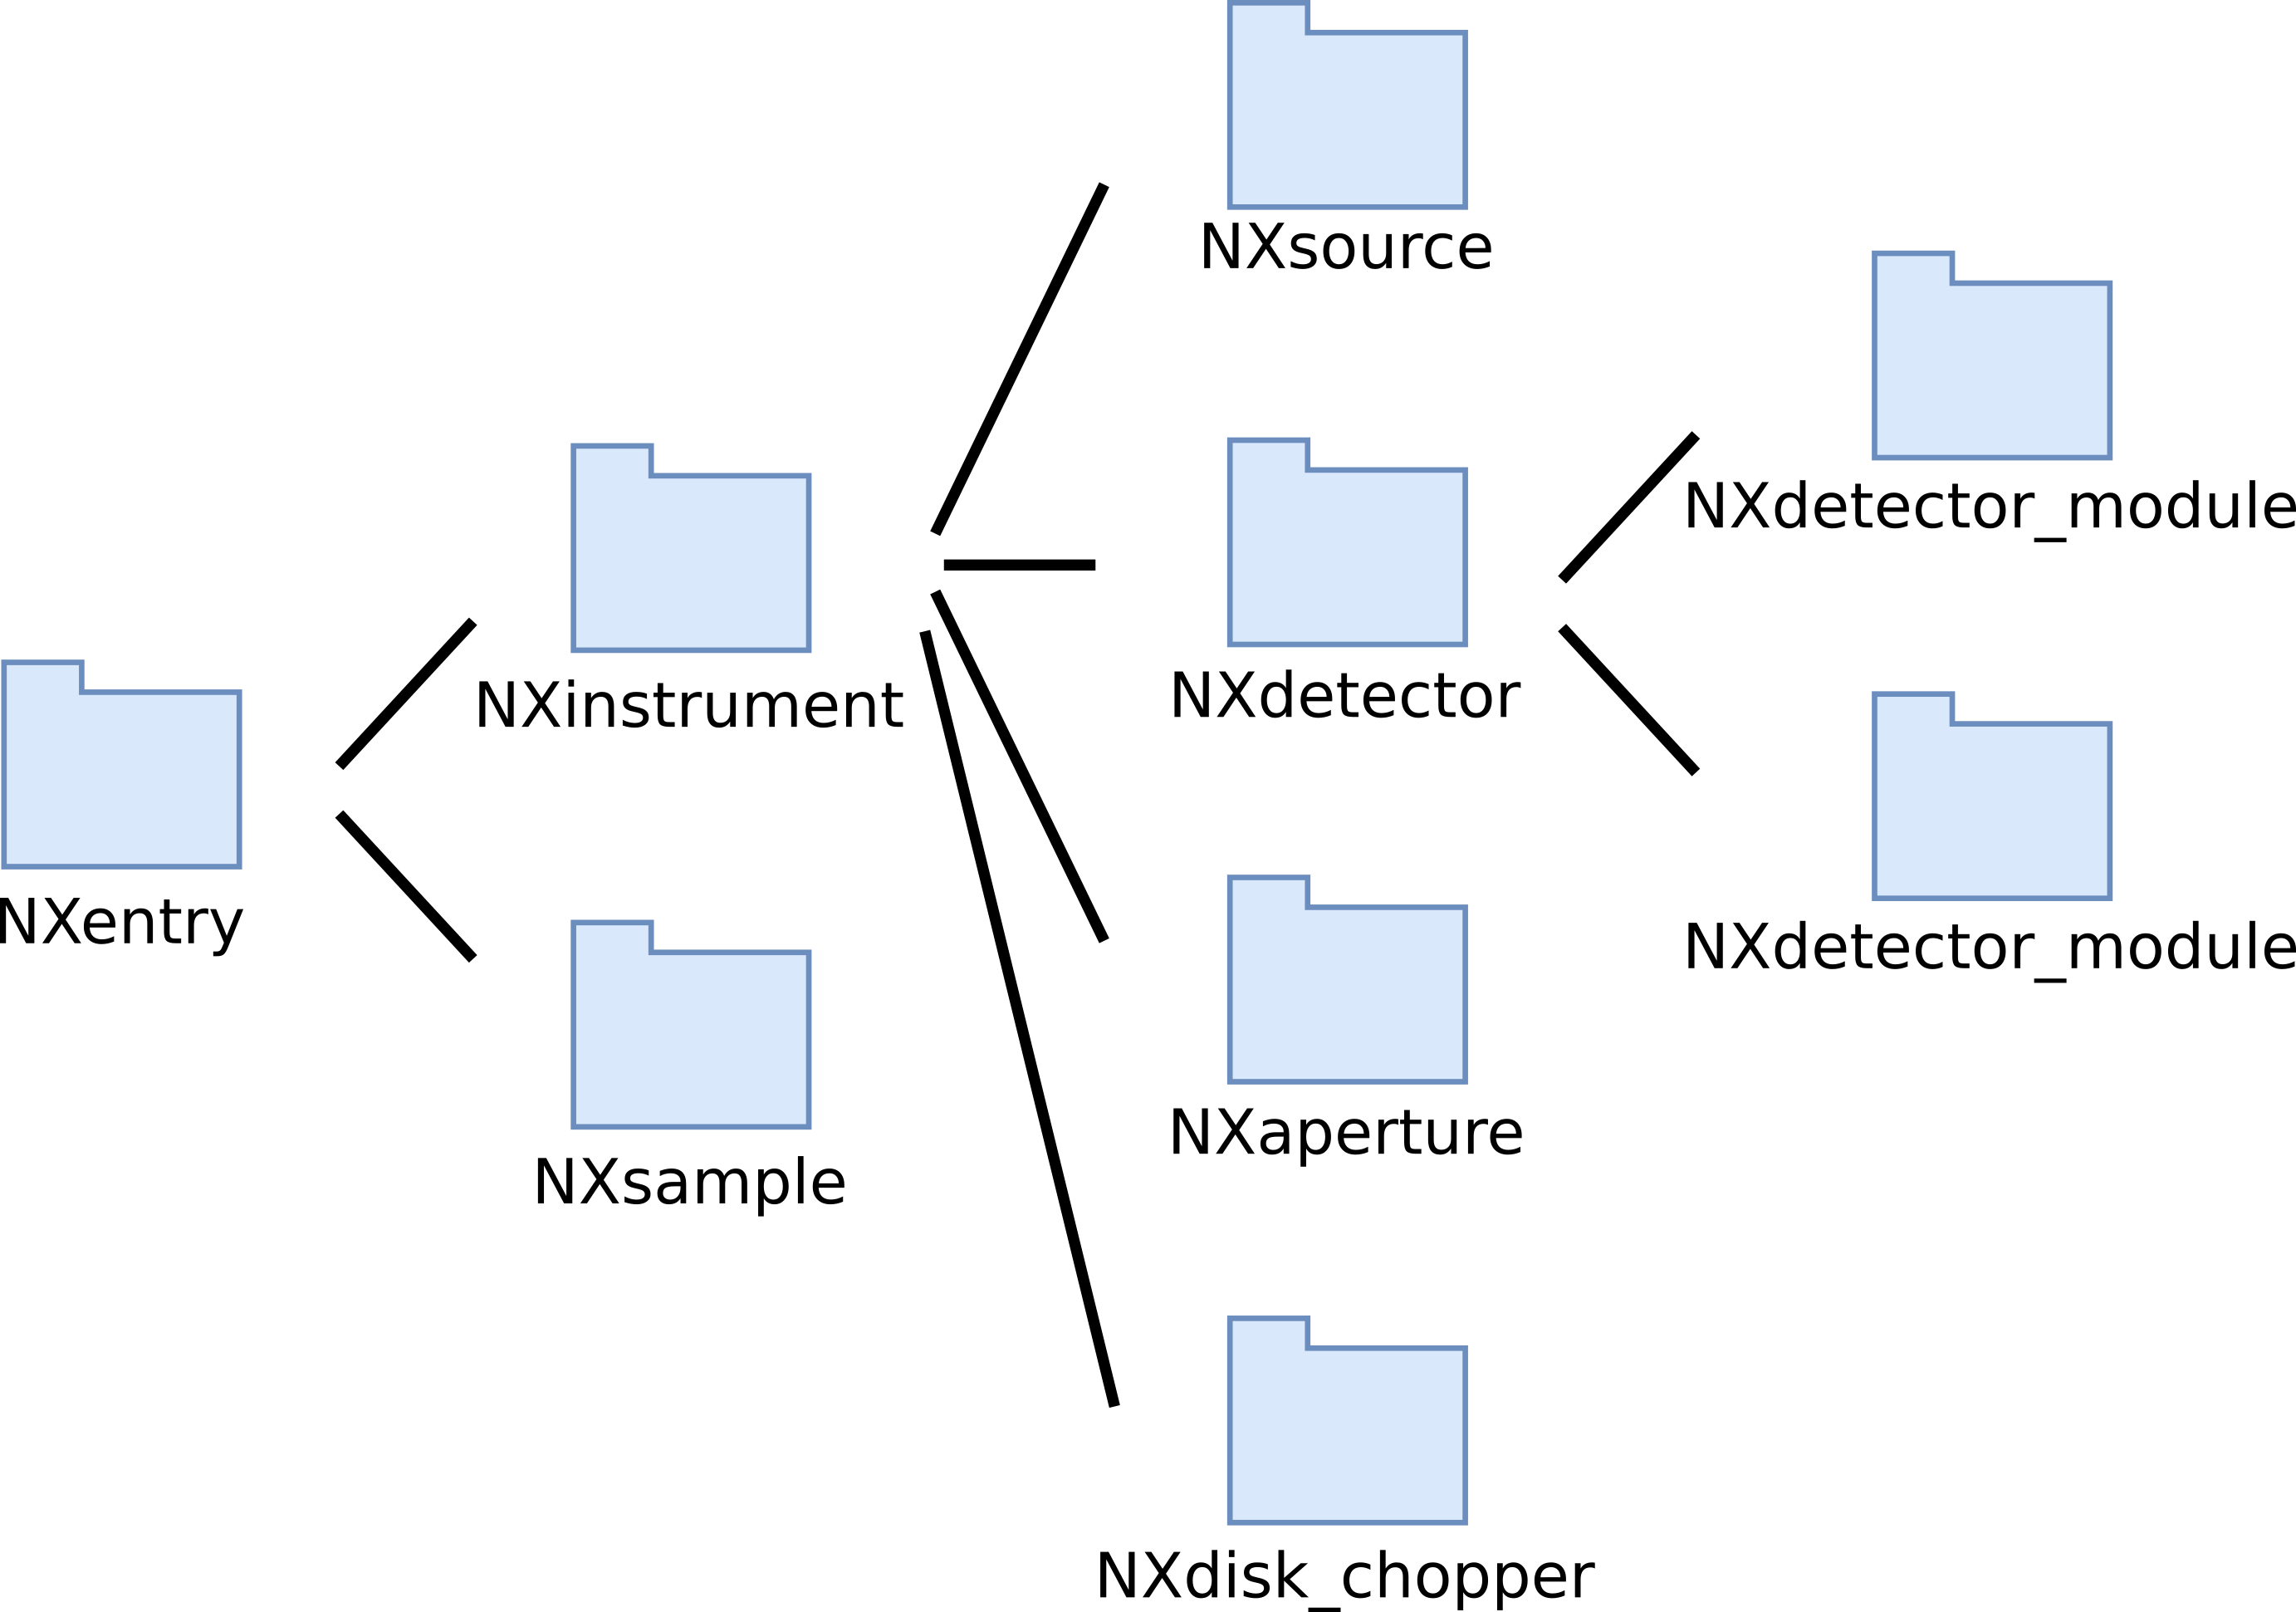
\includegraphics[width=0.6\linewidth]{instrument_arch.png}
\caption{A typical NeXus file layout}
\end{figure}

% What's a shape definition?

The NeXus file format was developed with the aim of:
\begin{itemize}
\item Creating a file format which is common to different neutron facilities.
\item Storing all experiment data in a single file.
\item Allowing experiment data to be loaded into a variety of different software tools.
\end{itemize}

NeXus is an extension of the popular HDF5 file format.

\iffalse
A recent addition to the NeXus standard means components that are used in experiments can specify shape definition to describe their placement, size and geometry. Transformations (NXtransformations) can be applied to these components when their position changes during or before the experiment.
\fi

\end{custombox}

\end{column}   
%%%%%%%%%% End of Column 1 %%%%%%%%%%

%%%%%%%%%% Start of Column 2 %%%%%%%%%%
\begin{column}{0.32\paperwidth}
\vspace{-10pt}

\begin{custombox}{The NeXus Constructor}
% pScientists typically have to seek out the aid of software developers in order to obtain configuration files that matched their specifications. This is currently being done manually by editing large JSON files which is both fragile as well as time-consuming for both parties involved.

The NeXus Constructor is a tool written with Qt for Python which allows scientists to create, edit and visualise NeXus files with minimal assistance. Such files can then be used for configuring the experiment control software in order to write real-time data. The layout of the NeXus Constructor interface consists of the following elements:

% Someone may not know what experiment control software does, what makes real-time data good, etc.

\begin{itemize}
\item Instrument View - A Qt3D pane that draws the experiment components in 3D. As NeXus files can contain information about a component's geometry and any transformations that may have been applied to it, translating this into something Qt3D can understand is fairly simple.
\item Component List - A list of the components in the NeXus file.
\item NeXus File Layout - An illustration of the hierarchical NeXus structure. Can't be used to see the values of the individual fields, but can serve as a tool through which you can check that the data has a sensible arrangement. Because the NeXus format is based on HDF5, the \texttt{h5py} library is able to interpret NeXus files so that we may display their layout in our application.
\end{itemize}

\begin{figure}
\caption{Screenshot of the NeXus Constructor}
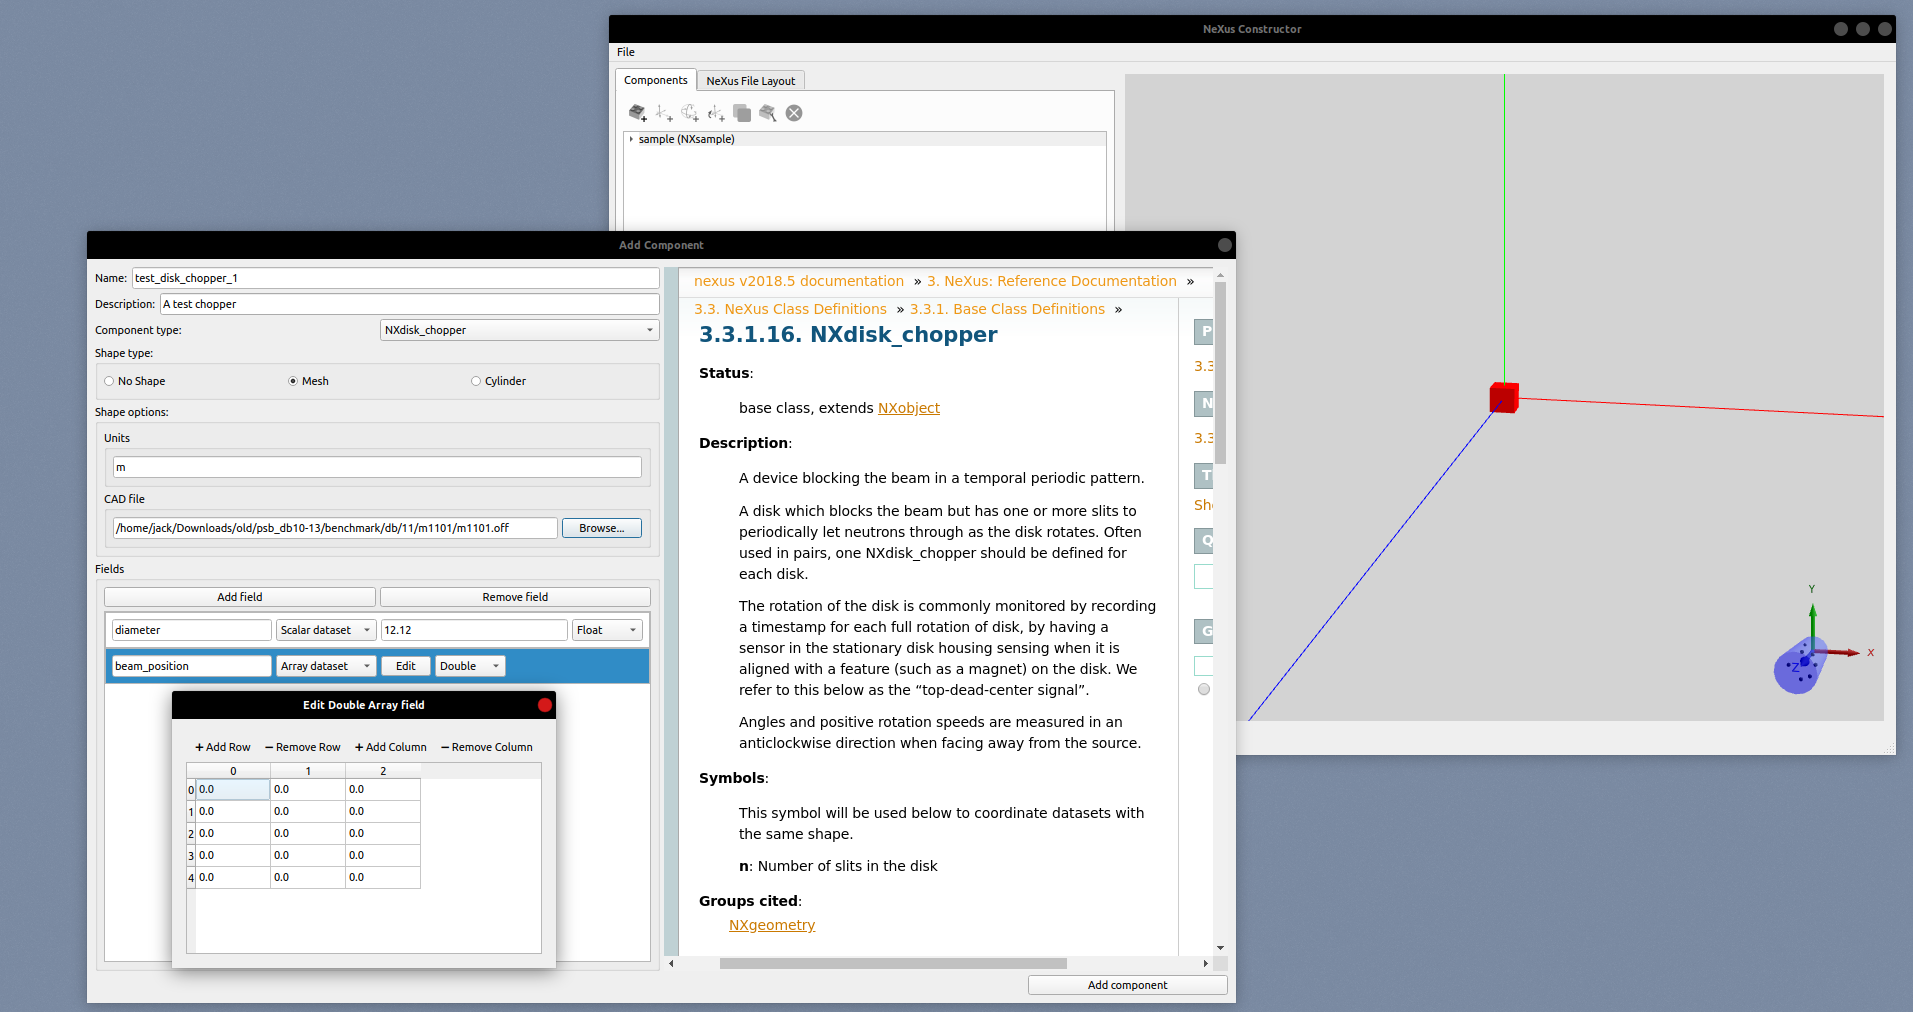
\includegraphics[width=\linewidth]{screenshot.png}
\end{figure}

The screenshot shows the main window of the NeXus Constructor and its "Add Component" dialog which allows users to add extra data in a NeXus file that describes the components that were present in an experiment.





\end{custombox}

\begin{custombox}{Technology}
\mysubtitle{Feature-Related}
\begin{itemize}
\item \texttt{pint} - Unit conversion. This comes in handy when drawing 3D objects from mesh files or NeXus files that contain geometry information but lack unit information. Pint can help enable validation and conversion for different types of units, as well as different types of different types of units (e.g. ``meter" and ``metres").
\item \texttt{h5py} - Reading from and writing to NeXus files. (This is also used by the \texttt{pandas} library.)
\item \texttt{silx} - Displaying the contents of NeXus files in a tree view.
\end{itemize}
\mysubtitle{Development-Related}
\begin{itemize}
\item \texttt{black} and \texttt{flake 8} - Code formatting and linting.
\item \texttt{pre-commit} - Code hygiene.
\item \texttt{pytest} and \texttt{pytest-cov} - Testing with coverage output.
\item \texttt{pytest-qt} - Simulating user interactions in order to check that the user clicking on object X triggers event Y. Especially useful when combined with \texttt{parameterize} to ensure that every \textit{possible} combination of actions that should lead to Y does indeed lead to Y.
\end{itemize}

\end{custombox}


\begin{tcolorbox}[enhanced,width=\linewidth,height=5cm,arc=5mm,
       interior style={fill overzoom image*={}{G04compressor.jpg}}]
\end{tcolorbox}

\end{column}
%%%%%%%%%% End of Column 2 %%%%%%%%%%  
\begin{column}{0.32\paperwidth}
\vspace{-10pt}

\begin{tcolorbox}[enhanced,width=\linewidth,height=14cm,arc=5mm,
       interior style={fill overzoom image*={}{essaerial.jpg}}]
\end{tcolorbox}

\begin{custombox}{Qt for Python}
We are using Qt for Python(PySide2) for the NeXus Constructor's graphical user interface. These are the official bindings for Qt 5 C++ API, provided by the Qt company.
\bigskip
There are two main methods of using Qt in Python, the more common "Widgets" framework or Qt-Quick which uses a markup language called QML.
We are taking the Qt-Widgets approach to developing the NeXus constructor, as the tooling for Qt-Quick/QML seems to be a bit lacking and some of the bindings are not as pythonic, and rather use C++-like idioms. Widgets also look more native to the OS running them. The main advantage QML provides is it's scaling for high-resolution displays or mobile devices.
\bigskip
Since version 5.12 PySide2 has included the Qt3D module in Qt5. We are utilising this with our 3d View of components in the neutron experiments. Qt3D provides a high-level interface to OpenGL which allows us to display the geometry information of components as well as an animated pulsed neutron beam. Qt3D's entity framework is similar to other GUI frameworks and 3D engines, such as unity. This means all the textures, meshes and transformations can be stored with a single entity in the Qt3d view, which is convenient for easily changing aspects of the 3d object. 
\bigskip
\begin{figure}
\caption{Qt3D's element inspector}
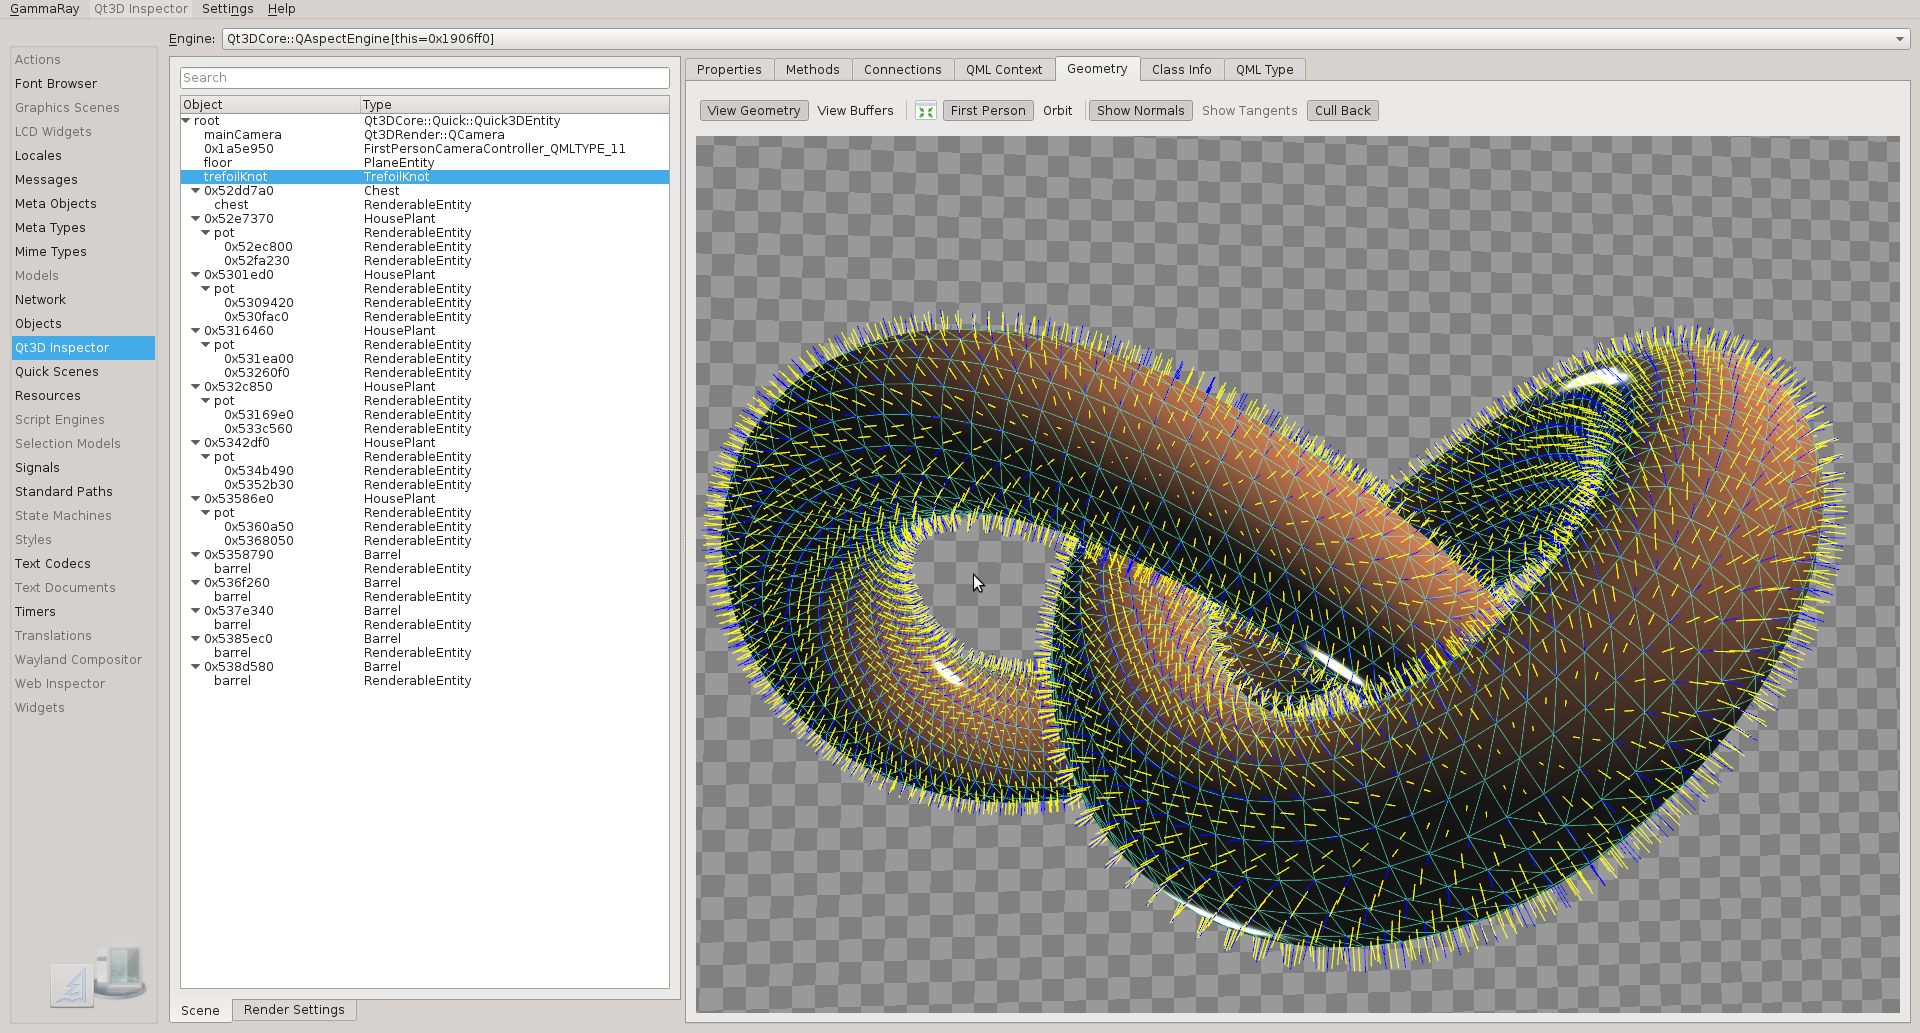
\includegraphics[width=\linewidth]{qt3d.png}
\end{figure}
\bigskip

The code snippet below shows the usage of a typical Qt3D view in python. Qt3D provides some high-level geometry types for adding cylinders, meshes, spheres as well as several other shapes. This is all wrapping OpenGL, and in the future Qt have stated they will support other graphics engines such as DirectX12, Vulkan and Metal. Currently there is some limited support for vulkan using the QVulkanWindow with a QVulkanInstance.

\begin{minted}[
frame=lines,
framesep=2mm,
fontsize=\footnotesize,
linenos
]
{python}
from PySide2.QtGui import QGuiApplication, QMatrix4x4, QQuaternion, QVector3D, QWindow
from PySide2.Qt3DCore import Qt3DCore
from PySide2.Qt3DRender import Qt3DRender
from PySide2.Qt3DExtras import Qt3DExtras

class CylinderWindow(Qt3DExtras.Qt3DWindow):
    def __init__(self):
        super(CylinderWindow, self).__init__()
        # Camera
        self.camera().lens().setPerspectiveProjection(45, 16 / 9, 0.1, 1000)
        # For camera controls
        self.createScene()
        self.cam_controller = Qt3DExtras.QOrbitCameraController(self.rootEntity)
        self.cam_controller.setCamera(self.camera())
        self.setRootEntity(self.rootEntity)
        self.cylinders = []
        self.meshes = []
        self.transforms = []

    def createScene(self):
        # Root entity
        self.rootEntity = Qt3DCore.QEntity()
        # Material
        self.material = Qt3DExtras.QPhongMaterial(self.rootEntity)

    def add_cylinder(self, radius, length, x, y, z, rings=10, slices=10):
        cylinder_entity = Qt3DCore.QEntity(self.rootEntity)
        # Using built in Qt cylinder Mesh
        cylinder_mesh = Qt3DExtras.Qcylinder_mesh()
        cylinder_mesh.setRadius(radius)
        cylinder_mesh.setLength(length)
        cylinder_mesh.setSlices(rings)
        cylinder_mesh.setRings(slices)
        # Add transforms to move the shape
        cylinder_transform = Qt3DCore.QTransform()
        cylinder_transform.setTranslation(QVector3D(x, y, z))
        # Add components to 3D entity
        cylinder_entity.addComponent(cylinder_mesh)
        cylinder_entity.addComponent(self.material)
        cylinder_entity.addComponent(cylinder_transform)
        # Add to list for easy access later        
        self.cylinders.append(cylinder_entity)
        self.meshes.append(cylinder_mesh)
        self.transforms.append(cylinder_transform)
\end{minted}


\end{custombox}

\begin{custombox}{Qt3D in the NeXus Constructor}
Qt3D provides a high-level interface to OpenGL which allows us to display instrument components in 3D. Qt3D's entity framework is similar to other GUI frameworks and 3D engines such as Unity. This means all the textures, meshes, and transformations can be stored with a single entity in the Qt3D view. This is convinient because the NeXus Constructor allows for applying transformations and changing the size of cylinder meshes and with Qt3D we can facilitate these changes without having to build the entire entity from scratch. 
\bigskip
\iffalse
\begin{figure}
\caption{Qt3D's element inspector}
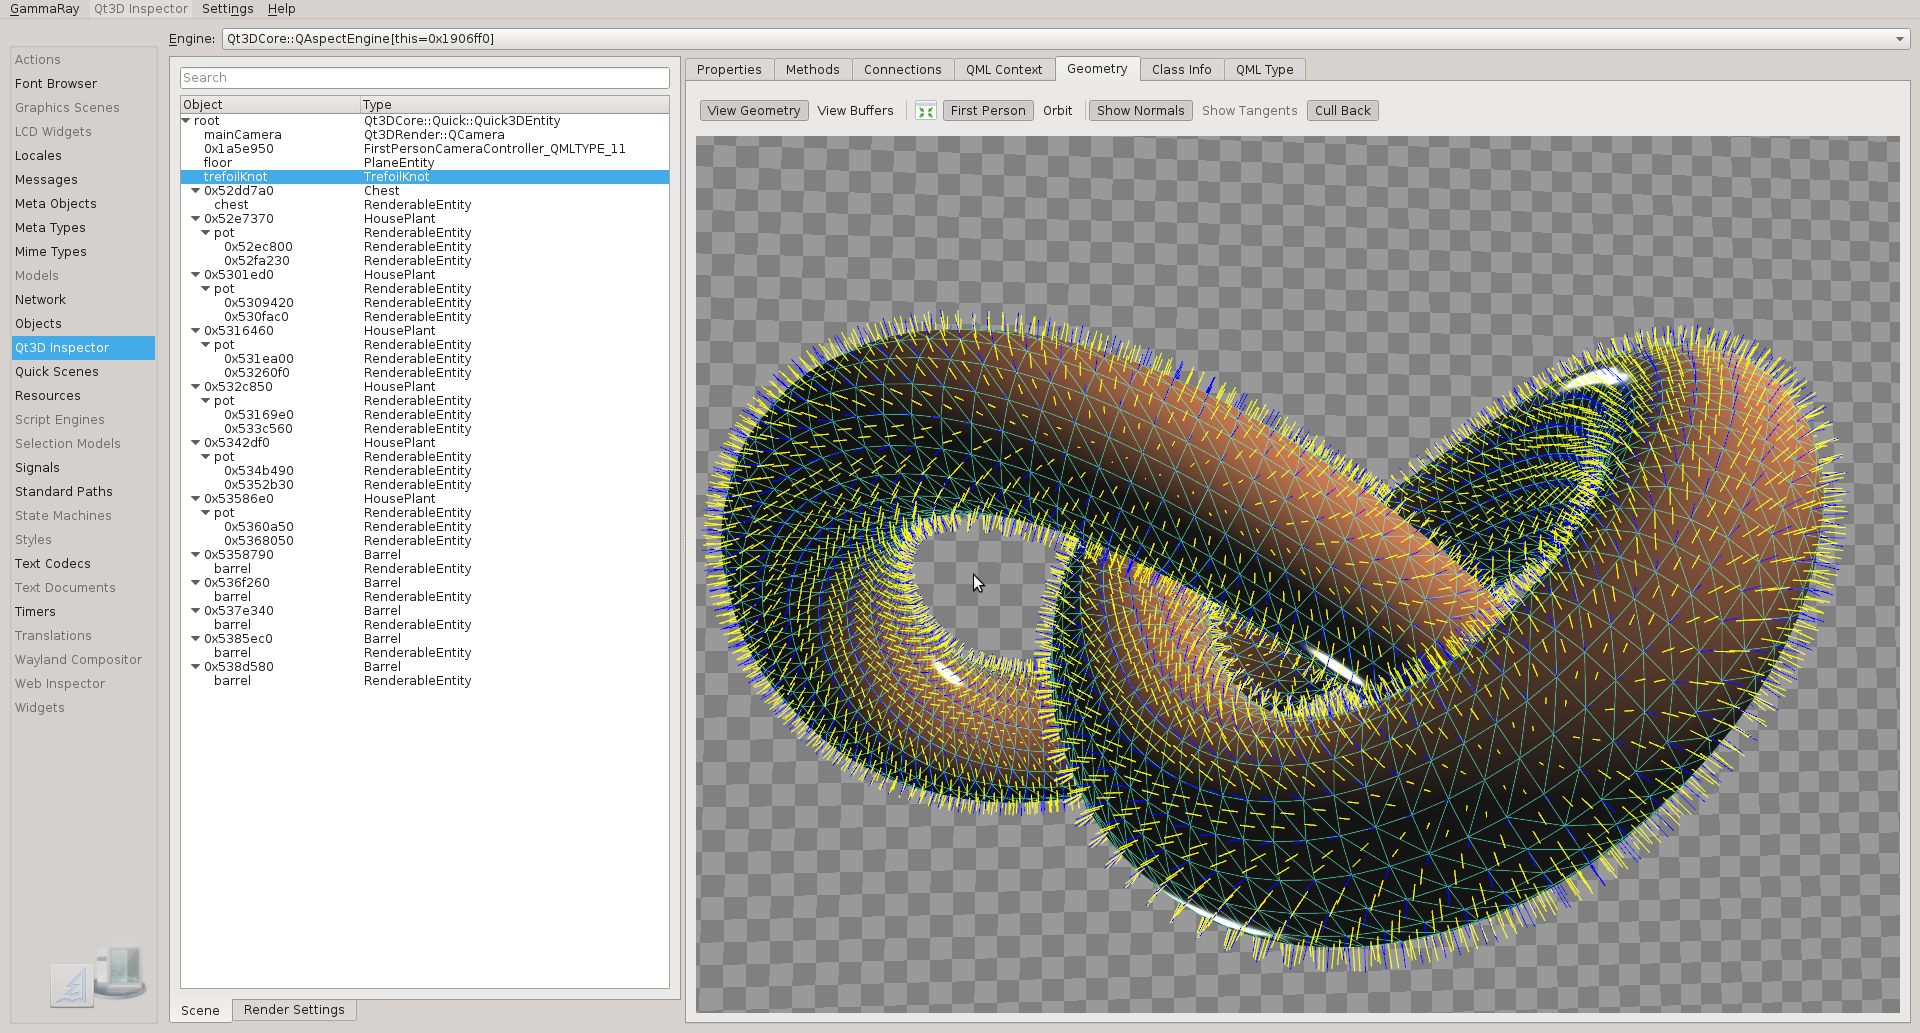
\includegraphics[width=\linewidth]{qt3d.png}
\end{figure}
\fi
\bigskip

\end{custombox}

\vspace{230pt}

\begin{tcolorbox}[enhanced,width=\linewidth,height=17cm,arc=5mm,
       interior style={fill overzoom image*={}{beamon.png}}]
\end{tcolorbox}
\vspace{-1.5cm}
\begin{center}
\color{white}\LARGE\textbf{https://www.isis.stfc.ac.uk\\https://europeanspallationsource.se}
\end{center}
\end{column}
\end{columns}
\end{frame}
\end{document}
 
